% 
% Annual Cognitive Science Conference
% Sample LaTeX Paper -- Proceedings Format
% 

% Original : Ashwin Ram (ashwin@cc.gatech.edu)       04/01/1994
% Modified : Johanna Moore (jmoore@cs.pitt.edu)      03/17/1995
% Modified : David Noelle (noelle@ucsd.edu)          03/15/1996
% Modified : Pat Langley (langley@cs.stanford.edu)   01/26/1997
% Latex2e corrections by Ramin Charles Nakisa        01/28/1997 
% Modified : Tina Eliassi-Rad (eliassi@cs.wisc.edu)  01/31/1998
% Modified : Trisha Yannuzzi (trisha@ircs.upenn.edu) 12/28/1999 (in process)
% Modified : Mary Ellen Foster (M.E.Foster@ed.ac.uk) 12/11/2000
% Modified : Ken Forbus                              01/23/2004
% Modified : Eli M. Silk (esilk@pitt.edu)            05/24/2005
% Modified: Niels Taatgen (taatgen@cmu.edu)  10/24/2006

%% Change ``a4paper'' in the following line to ``letterpaper'' if you are
%% producing a letter-format document.









\documentclass[10pt,letterpaper]{article}

\usepackage{cogsci}
\usepackage{pslatex}
\usepackage{apacite}
\usepackage{graphicx}
\usepackage{color}
\usepackage{amsmath}
\usepackage{multirow}
\usepackage{amssymb}
%\usepackage{url}
%\usepackage{hyperref}


 
\definecolor{Red}{RGB}{255,0,0}
\newcommand{\red}[1]{\textcolor{Red}{#1}}  


\title{ Lay theories of emotion in explaining behavior }
 
\author{{\large \bf Desmond C. Ong (dco@stanford.edu)} \\
{\large \bf Jamil Zaki (jzaki@stanford.edu))} \\
{\large \bf Noah Goodman (ngoodman@stanford.edu)} \\
  Department of Psychology, Stanford University, Stanford CA, USA 
}

\begin{document}

\maketitle

\begin{abstract}
Abstract

\textbf{Keywords:} 
Keywords
\end{abstract}

% Outline of paper

% More free-form
% Expt 1a) Emotions --> Actions
% Expt 1b) Generate cause of Actions. Coded into emotions, beliefs, situational factors, etc.

% More hypothesis driven
% Expt 2a) Actions / Expressions / Behavior, generate causes: Beliefs, Desire, Emotion, Situation factor
% Expt 2b) From 2a, for all actions/expressions/behavior, pick top b,d,e,s. Find endorsement rates of posterior using sliders.







%Talk about Malle's Cause vs. Reason. Intentional vs unintentional behavior

\red{[TODO: more setup]}


One hypothesis is that in our lay theories of behavior, there are two distinct processes that result in two types of behavioral responses (see Fig. \ref{ModelsOfBehaviorFig}a). The first of these processes is a rational decision making process in which an agent has a set of goals (``desires"), and a set of ideas on how to achieve those goals (often termed ``beliefs"). The agent then forms an intention to act upon his beliefs to achieve his desires, resulting in (intentional) action, as part of a ``belief-desire psychology" \cite{Dennett1989, Gopnik1997, Heider1958, Malle2011, Searle2001}. The second process, by contrast, relies on mere causality or ``impersonal causality" \cite{Heider1958}, and results in a second type of behavioral response. These behaviors could be caused by external situational factors, or as is often implicitly assumed by theories of folk psychology, the agent's emotions. Here, we make a distinction here between emotional expressions on one hand (e.g., crying), assumed to be caused only by emotions, and other unintentional behavior on the other (e.g., slipping on ice, snoring) that could be due to situational factors, and possibly emotions as well. Notably, in these theories of folk psychology, there is no place for emotions in the ``rational" decision making process that humans reason with when explaining the actions of others.
% Probably can say a bit more in the above paragraph when I read those papers.

A second hypothesis is that emotions do play an important role in the formation and execution of intentional action. Figure \ref{ModelsOfBehaviorFig}b posits a lay theory in which emotions are factored into the intentional decision making process. This approach been incorporated into psychological \cite<e.g., >{Schwarz2000emotion}, economic \cite<e.g., >{Loewenstein2003affect}, and philosophical \cite<e.g., >{Zhu2002emotion} theories of behavior, but it is unclear how a theory of folk psychology incorporates emotions into the lay model of decision making \cite{Ong2015AffCog}. A third possibility that we must also consider is that the distinction between intentional action and emotional expressions in the lay theory is needlessly strong (Fig. \ref{ModelsOfBehaviorFig}c), and that emotions, as well as beliefs and desires, impact an agent's intentional actions and emotional expressions. Indeed, emotional display rules \cite<e.g., >{Matsumoto1990} and deceptive strategies \cite<e.g., >{Depaulo2003} do impact an agent's displayed emotional expressions, and might very well be an important factor in lay explanations of behavior. However, we (as have many theorists before us) reject the notion that all instances of emotional expressions are intentional, and hence should not be a subset of intentional action.


\begin{figure}[htb!]
\begin{center}
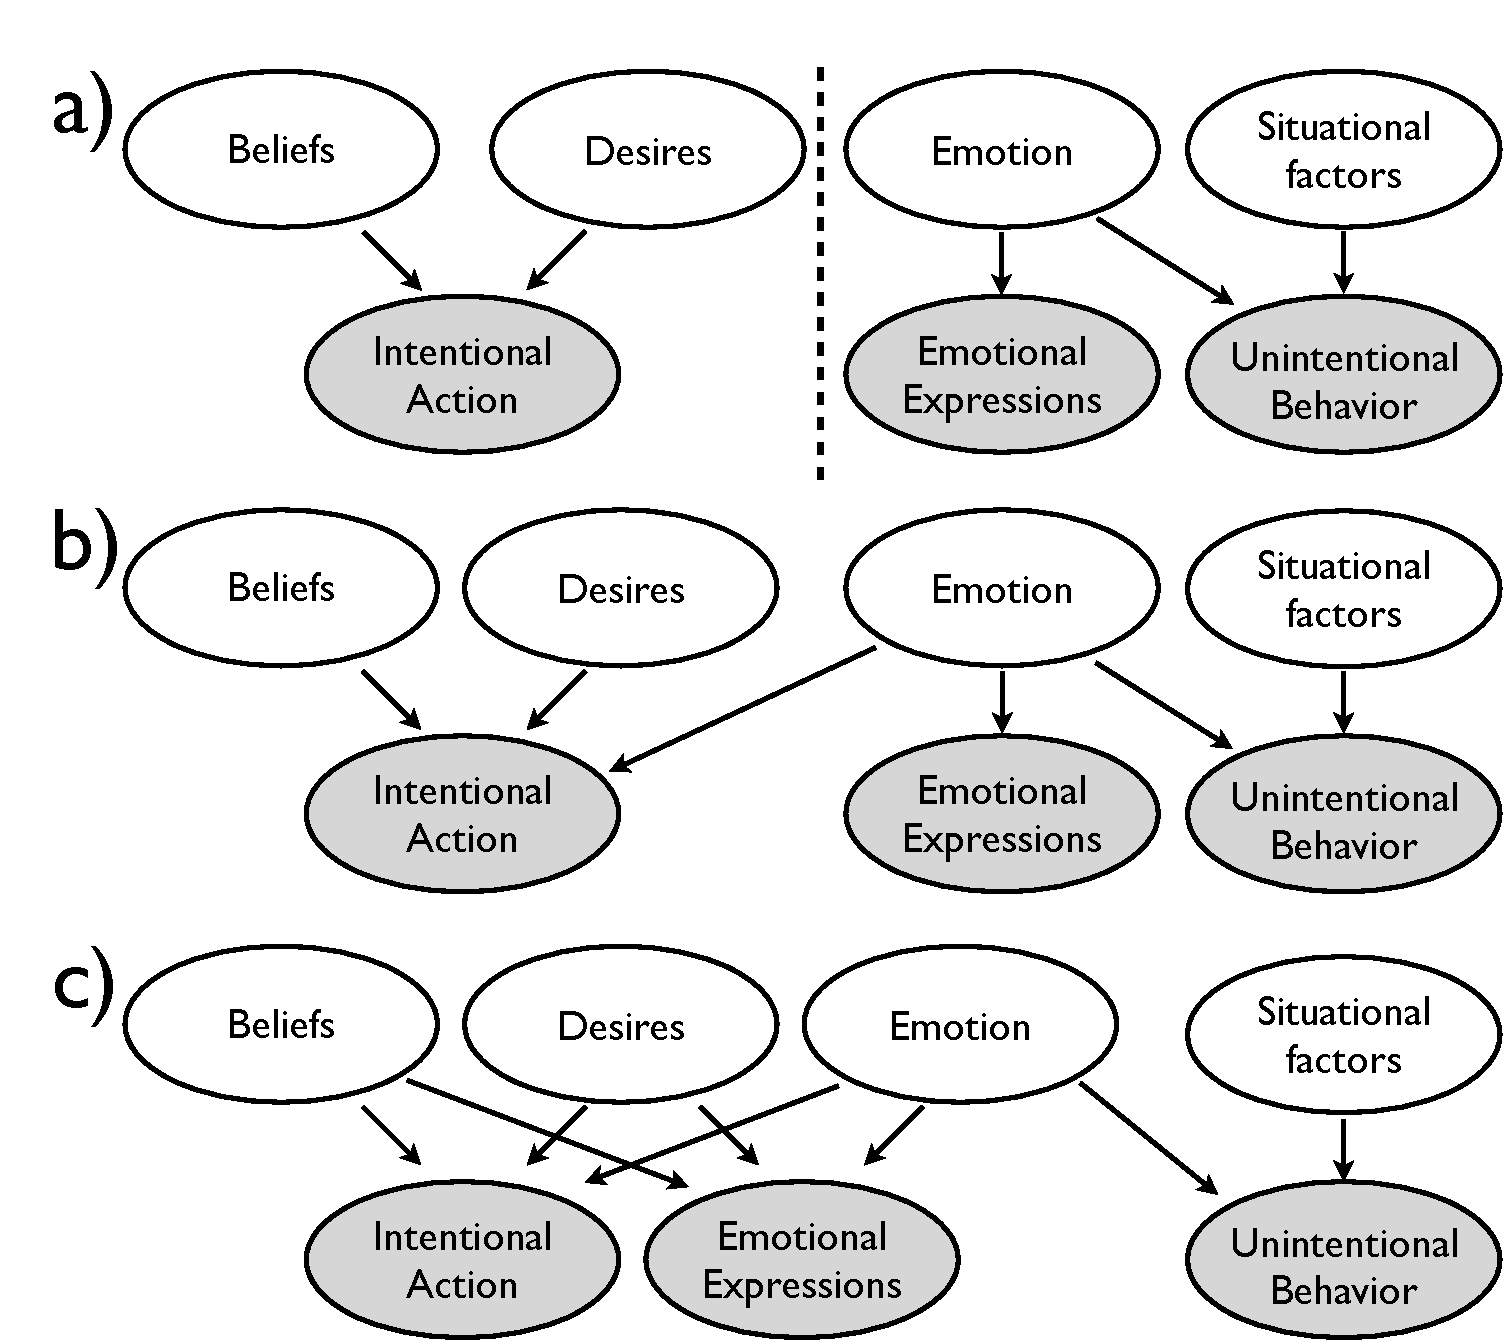
\includegraphics[width=1\columnwidth]{images/model1.pdf} 
\end{center}
\caption{ Possible lay theories of behavior. (a) There are two distinct types of behavioral responses; the rational decision-making process that goes from beliefs and desires to intentional action, and unintentional behavior and emotional expressions that are caused by situational factors and emotions. The latter process is governed by simple causality, without the need for an agent's intentionality. (b) Emotions do factor into the intentional decision making process, but there still exists emotional expressions and other unintentional behavior that are unaffected by beliefs and desires. (c) There is no sharp distinction between intentional action and emotional expressions in that both are affected by beliefs, desires and emotions.  }
\label{ModelsOfBehaviorFig}
\end{figure}



% TODO: finish this part

In this paper we provide some explorations of how emotions are incorporated into lay belief-desire psychology. We show that ... \red{[TODO: finish this part]}




In order to test this, we elicited what types of behavior were most likely given ...


%%%%


\section{Study 1a: Emotions to Actions}

	In Study 1a\footnote{https://github.com/desmond-ong/shakespeare/Cogsci}, we elicited participants' free-response nominations of emotion-caused actions. We then obtained judgments of the counterfactual likelihood (i.e., how likely were their nominated actions, if the agent had not felt the emotion).

% Expt 1a) Emotions --> Actions
% Expt 1b) Generate cause of Actions. Coded into emotions, beliefs, situational factors, etc.

\subsubsection{Participants and Procedures.} 
We recruited 100 participants through Amazon's Mechanical Turk (AMT). Participants saw statements of the form ``Bob \underline{\hspace{3em}} because he was [\textbf{emotion}]", and were asked to give sentence completions. The presented \textbf{emotion} was one of: \{happy, calm, anger, sad, surprised\}\footnote{We chose a high-arousal positive valence (``happy"), a low-arousal positive valence (``calm"), a high-arousal negative valence (``anger"), a low-arousal negative valence (``sad"), and a high-arousal neutral valence (``surprised") emotion.}. On each page, participants saw only one emotion, and gave 5 different completions (for a total of 25 completions). The emotions were presented in a random order; names were randomized on every sentence.

% do we use the counterfactual judgments?
After participants had given completions to all 5 emotions, they were then presented their answers, and asked to rate the likelihood of the counterfactual: ``You wrote that `\textit{Bob [cried] because he was [sad]}'. If Bob was not feeling [sad], would he still have [cried]?" Participants gave responses on a 7 point Likert scale from ``Very Unlikely" to ``Very Likely". 


%\multirow{2}{*}{text}

\subsubsection{Results.} 
Similar free-responses were grouped together (e.g., ``smiled", ``smiled widely", and ``beamed"). The top 5 responses, with nomination counts, for each emotion are given in Table \ref{Study1aResultsTable}. Many of the responses for Anger were of the form ``hit X", where X is an object or person. Note that, as expected, the majority of these top responses would easily be judged to be ``emotional expressions": some notable exceptions are ``killed himself\footnote{It is unfortunate that this is one of the modal responses for what an agent will do when he is sad...}", ``slept", and ``sat down".


\begin{table}
\scalebox{0.80}{
\begin{tabular}{l l l l l}
\textbf{Happy} & \textbf{Calm} & \textbf{Sad} & \textbf{Anger} & \textbf{Surprised} \\
%\hline
smiled: 63 & relaxed: 50 & cried: 97 & ``hit X": 56 & jumped: 65 \\
laughed: 51 & slept: 46 & frowned: 17 & yelled: 54 & laughed: 41 \\
\multirow{2}{*}{jumped: 42} & \multirow{2}{*}{sat down: 32} & killed & \multirow{2}{*}{screamed: 21} & \multirow{2}{*}{screamed: 30} \\
& & himself: 13 & & \\
danced: 22 & smiled: 26 & slept: 13 & cried: 15 & yelled: 25 \\
cried: 21 & sighed: 10 & yelled: 13 & cursed: 12 & smiled: 23 \\
\end{tabular}
}
\caption{ Action nominations from emotions (Study 1a). Top 5 responses for each emotion, with nomination counts. The most common responses for anger were variants of ``hit X", where X is an object or person (of these, the modal response was: ``punched the wall"). }
\label{Study1aResultsTable}
\end{table}



The more often a particular action $a$ is nominated for emotion $e$, presumably, the more characteristic is action $a$ of emotion $e$. Hence, we should expect that these commonly nominated actions $a$ would be less likely to happen in the absence of emotion $e$. In order to test this, we regressed participants' counterfactual likelihood ratings (i.e., how likely is the action to occur if the emotion was absent, $P(A | \neg E)$) against the frequency of that action being nominated across the sample, with random intercepts by participant and emotion. We find that, across all emotions, the more frequently an action is nominated, the less likely participants rate it to occur in the absence of the emotion $(b = -0.0084, 95\% \text{ CI}: [-0.0108, -0.0060], t=-6.82, p<0.001$; See Fig. \ref{Study1aResultsFig}). Thus, the modal nominated actions are judged less likely to occur in the absence of the corresponding emotions, and might thus be seen as more characteristic of their corresponding emotions: we shall use this result in Study 1b.



\begin{figure}[htb!]
\begin{center}
	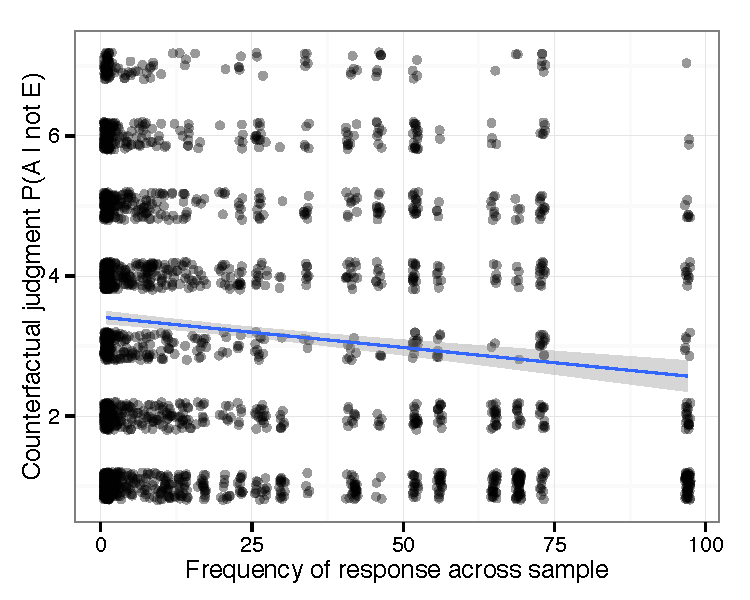
\includegraphics[width=1\columnwidth]{images/study1a_results.pdf}
\end{center}
\caption{ Study 1a Results. Individual counterfactual likelihood ratings ($P(A | \neg E)$) against frequency of an action's nomination across the sample. Data points are transparent and jittered for clarity. }
\label{Study1aResultsFig}
\end{figure}


\section{Study 1b: Causes of Actions}

	In Study 1b, we took the top actions nominated from Study 1a, and asked a separate group of participants to give explanations for those actions. The top actions from Study 1a are judged to be less likely to occur in the absence of the emotion, and hence are presumably more characteristic of the emotions, (Study 1a). Hence, if Model 1 (Fig. \ref{ModelsOfBehaviorFig}a) were correct, we should only expect explanations due to emotions (and perhaps, situational factors).


\subsubsection{Participants and Procedures.} 
In a similar manner to Study 1a, we recruited 100 participants through Amazon's Mechanical Turk (AMT). This time, participants saw statements of the form ``Bob [\textbf{action}] because \underline{\hspace{3em}}" (i.e., the reverse of Study 1a), and were asked to complete the sentence. The presented \textbf{action} was one of fifteen possible actions drawn from the most popular nominations from Study 1a (i.e., the 15 unique actions in Table \ref{Study1aResultsTable}: ``punched the wall" was used in place of ``hit X"). Participants gave 1 completion per action and saw the actions in a random order.
% do we use the counterfactual judgments?

\subsubsection{Results.} 
The free-response completions were coded into one of five categories: (a) ``\textbf{Emotion}" (if there was a mention of an emotion word), (b) ``\textbf{Cause of Emotion}" (if there was a mention of an event that would cause an emotion, e.g., ``his dog died"), (c) ``\textbf{Physical state}" (if the explanation references a physical state like tiredness or pain), (d) ``\textbf{Mental state}" (if the explanation references a desire or a belief); (e) ``\textbf{Situation}" (for enabling and other situational factors). 

The distribution of coded free-responses is given in Figure \ref{Study1bResultsFig}. \red{[TODO: write this next part more nicely and maybe some stats]} basically we should expect all explanations to be Emotion (and maybe + Cause of Emotion), but we see a huge range of responses across the board, invoking physical and mental state attributions, as well as other situational factors.

\begin{figure}[htb!]
\begin{center}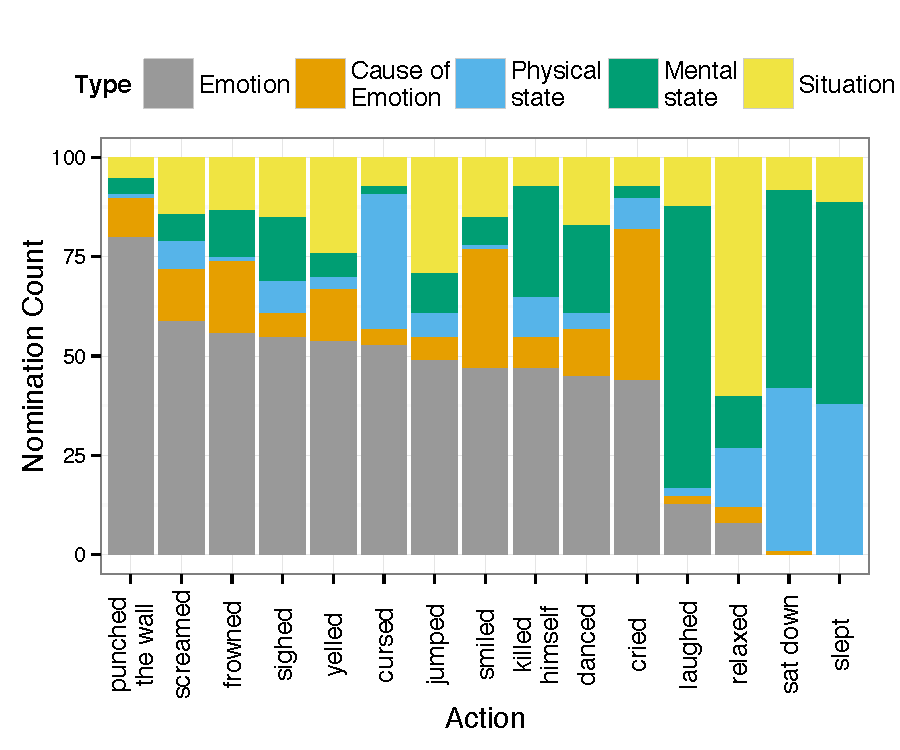
\includegraphics[width=1\columnwidth]{images/study1b_codePlot.pdf}\end{center}
\caption{ Results of Study 1b. We plot the number of nominations that fall into each explanation type for each action. }
\label{Study1bResultsFig}
\end{figure}


\section{Study 2: }


\subsubsection{Participants and Procedures.} 


% intentional actions after Malle 1999
%watered his new plants
%invited Sue to have lunch
%stole a pound of peaches
% drove above the speed limit -- ambiguous

% smiled
% cried
% yelled

% slipped and fell
% snored in his sleep
% stubbed his toe


\subsubsection{Results.} 





\section{Discussion}

Discuss

\section{Acknowledgments}

This work was supported in part by an A*STAR National Science Scholarship to DCO and by \red{[TODO:] XXX to NDG}.


\bibliographystyle{apacite}

\setlength{\bibleftmargin}{.125in}
\setlength{\bibindent}{-\bibleftmargin}

\bibliography{shakespeare_cogsci}





\end{document}
